\documentclass[a4paper,12pt]{amsart}

\newcommand{\ZZ}{\mathbb{Z}}
\newcommand{\RR}{\mathbb{R}}
\newcommand{\CC}{\mathbb{C}}
\newcommand{\PP}{\mathbb{P}}
\newcommand{\bfx}{\mathbf{x}}
\newcommand{\bfy}{\mathbf{y}}
\newcommand{\bfb}{\mathbf{b}}
\newcommand{\vx}{\begin{bmatrix}
		x_1\\
		\vdots\\
		x_n
\end{bmatrix}}
\newcommand{\vA}{\begin{bmatrix}
		A\\
		-A\\
		-I
\end{bmatrix}}
\DeclareMathOperator{\Hom}{Hom}
\DeclareMathOperator{\Spec}{Spec}

\usepackage[top=1in, bottom=1in, left=1in, right=1in]{geometry}
\usepackage{amsmath, amssymb}
\usepackage{amsthm}
\usepackage{dsfont}
\usepackage{enumerate}
\usepackage{graphicx}
\usepackage{subcaption}


\title{MATH7670 Lecture Notes}
\author{}


\date{January 24, 2019}
\begin{document}
\maketitle
\newtheorem{Lemma}{Lemma}
\newtheorem{Proposition}{Proposition}[section]
\newtheorem{Theorem}{Theorem}[section]
\newtheorem{Corollary}{Corollary}
\newtheorem*{Conjecture}{Conjecture}

\theoremstyle{definition}
\newtheorem*{Problem}{Problem}
\newtheorem*{Def}{Definition}
\newtheorem{Eg}{Example}

\theoremstyle{remark}
\newtheorem*{Remark}{Remark}
\newtheorem*{Caution}{\bf{Caution}}
\newtheorem*{Fact}{Fact}

%---This is the beginning of the document---

\section{Lecture 01}

What is a toric variety(over $\CC$)? simplest: $\PP^n$, also $\PP^{n_1}\times\PP^{n_2}\times\dots\times\PP^{n_r}$(via Segre embdedding).

\begin{Eg}[Hirzebruch surface]
A polygon
\begin{figure}[h]
\centering
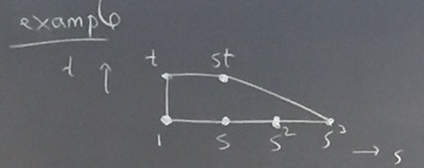
\includegraphics[width=0.7\textwidth]{pic/lec01pic01}
\end{figure}
\begin{align*}
\varphi:\mathbb{A}^2_{s,t}&\rightarrow\PP^5\\
(s,t)&\mapsto(1,s,s^2,s^3,t,st)
\end{align*}
Consider
\begin{equation*}
\overline{\varphi(\mathbb{A}^2)}=X\subseteq\PP^5.
\end{equation*}
$X$ is an example of a toric variety.
The edges correspond to curves $C_1,\dots,C_4$ on $X$, $C_1\cap C_2=\text{pt}$, $C_2\cap C_3=\text{pt}$, etc. $\text{Pic}X$ is generated by $[C_1],[C_2]$
\end{Eg}
Toric varieties allow explicit constructions of many concepts in A.G.
\begin{itemize}
\item singularities, smoothness, resolution of singularities 
\item divisors, geometry of divisors $\text{Pic}X$, $\text{Cl}X$.
\item cohomology of divisors
\item vector bundles, projective bundles, sheaf of differentials
\item  Serre duality, Riemann-Roch
\end{itemize}

Special features:
\begin{itemize}
\item defined using: cones, fans, polyhedron
\item action of the torus
\begin{equation*}
T=(\CC^*)^n.
\end{equation*}
\item homogenerous coordinates on a toric variety.
\end{itemize}

\begin{Caution}
Our toric varieties are always normal.
\end{Caution}
First few weeks:
\begin{itemize} 
\item cones, F-M,
\item affine toric varieties: define/ideals/points/singularities, maps, T-action.
\item projective, more general, toric varieties
\end{itemize} 
\subsection{Cones}
Let $V$ be a finite dimensional $\RR$-vector space.
\begin{Def}
Let $S\subseteq V$ be a subset, nonempty.
\begin{enumerate}
\item $S$ is a \textbf{(convex) cone} if $\forall \bfx,\bfy\in S$, $\forall \alpha,\beta\in\RR$, $\alpha,\beta\geq 0$, then $\alpha \bfx+\beta \bfy\in S$.
\item $S$ is a \textbf{convex set} if $\forall \bfx,\bfy\in S$, $\forall \alpha,\beta\in\RR$, $\alpha,\beta\geq 0$, $\alpha+\beta=1$, then $\alpha \bfx+\beta \bfy\in S$.
\end{enumerate}
\end{Def}
\begin{Eg}Some examples when $V=\RR^2$:
\begin{enumerate}
\item A convex cone:
\begin{figure}[h]
\centering
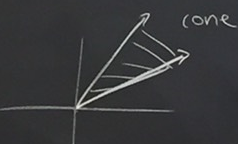
\includegraphics[width=0.7\textwidth]{pic/lec01pic02a}
\end{figure}
\item Convex sets:
\begin{figure}[h]
\centering
\begin{subfigure}{.5\textwidth}
  \centering
  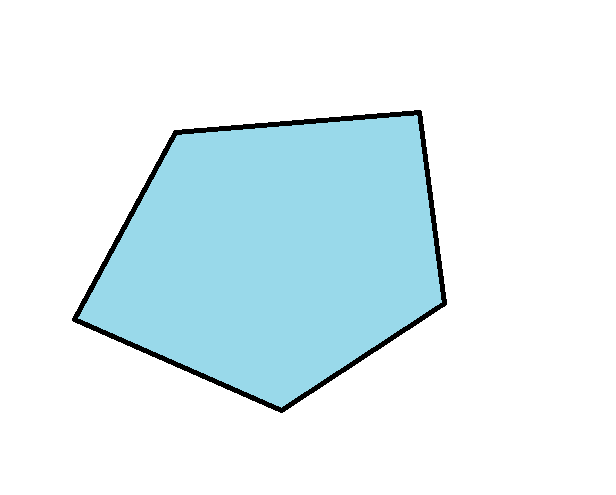
\includegraphics[width=.7\linewidth]{pic/lec01pic02b}
  \caption{A polygon}
  \label{fig:sub1}
\end{subfigure}%
\begin{subfigure}{.5\textwidth}
  \centering
  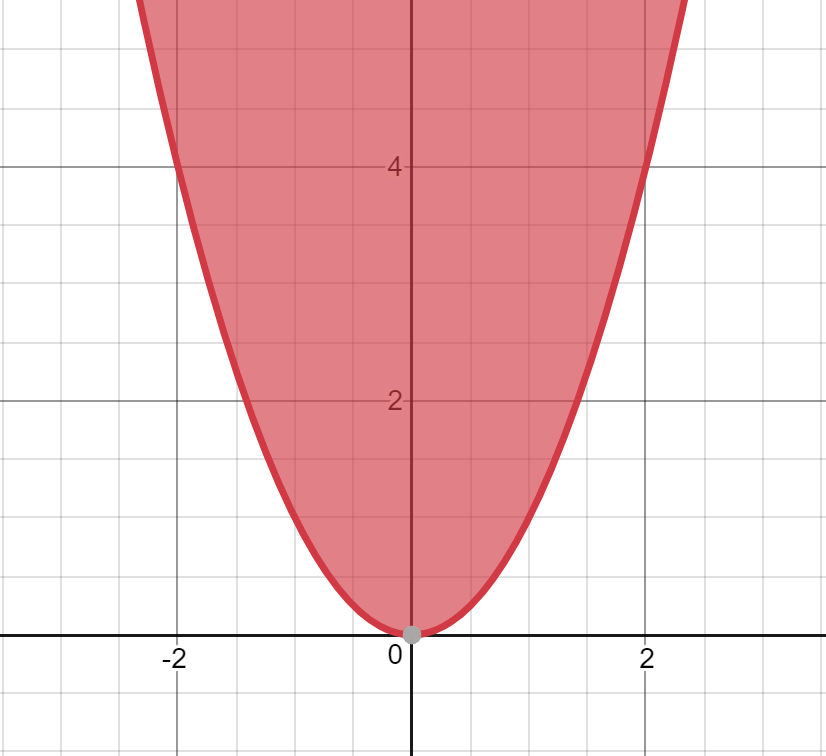
\includegraphics[width=.7\linewidth]{pic/lec01pic02c}
  \caption{$y\geq x^2$}
  \label{fig:sub2}
\end{subfigure}
\label{fig:test}
\end{figure}
\end{enumerate}
\end{Eg}

\begin{Eg}Key examples:
\begin{enumerate}
\item If $A\in \RR^{m\times n}$, write $A=[A_1, A_2\dots, A_n]$, define
\begin{align*}
\text{vcone}(A)&:=\{x_1A_1+\dots+x_nA_n\in\RR^n,x_1,\dots,x_n\geq 0\}\\
&=\{A\bfx\in\RR^n: \bfx\geq 0, \bfx\in \RR^n\}
\end{align*}
A cone of this form is called finitely generated or V-cone.
\item obtain cone via intersections of half-spaces. If
\begin{align*}
B=\begin{bmatrix}
B_1\\
\vdots\\
B_d
\end{bmatrix}, B_i\in(\RR^n)^{*}
\end{align*}
Define
\begin{align*}
\text{hcone}(B)&:=\{\bfy\in(\RR^n)^{*}:\langle B_1,\bfy \rangle=B_1\bfy\leq 0,\dots,\langle B_n,\bfy \rangle=B_n\bfy\leq 0\}\\
&=\{\bfy\in(\RR^m)^*:B\bfy\leq 0\}
\end{align*}
\item if $A\in\RR^{m\times n}$, define
\begin{equation*}
\text{conv}(A):=\{x_1A_1+\dots+x_nA_n:x_i\geq 0,\sum x_i=1\}
\end{equation*}
A set of this form is a polytope.
\item if $A\in\RR^{m\times n}$, $\bfb\in\RR^m$
\begin{equation*}
P(A,\bfb):=\{\bfx\in\RR^n:A\bfx\leq \bfb\}
\end{equation*}
A set of this form is a polyhedron.
\end{enumerate}
\end{Eg}
\begin{Def}[Key construction: dual cone]
If $\sigma\in V$ is a cone, define its \textbf{dual cone}
\begin{align*}
\sigma^{\vee}=\{\bfy\in V^{*}:\langle \bfy,\bfx\rangle\leq 0, \forall \bfx\in\sigma\}.
\end{align*} 
(Check: $\sigma^{\vee}$ is also a cone.)
\end{Def}

\begin{Eg}
$V=\RR^2$. Let $\sigma=\text{cone}(A_1,A_2)$. Then $\sigma^{\vee}=\text{cone}(A_1^{\perp},A_2^{\perp})$.
\begin{figure}[h]
\centering
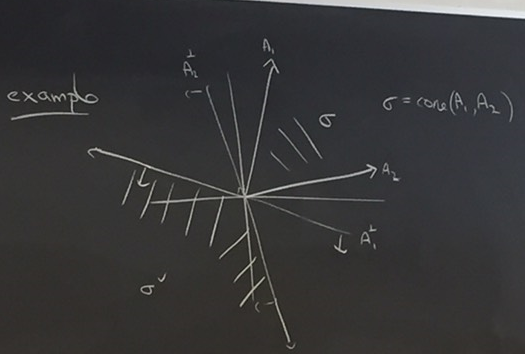
\includegraphics[width=0.7\textwidth]{pic/lec01pic03}
\end{figure}
\end{Eg}
\begin{Remark}
if $\sigma=\text{vcone}(A)$, $A\in\RR^{m\times n}$, then $\sigma^{\vee}=\text{hcone}(A^{T})$. This is because
\begin{align*}
\sigma^{\vee}&=\{\bfy\in(\RR^m)^*:\langle \bfy,\bfx \rangle\leq 0,\forall \bfx\in \sigma\}\\
&=\{\bfy: \langle \bfy,A_1 \rangle\leq 0,\dots,\langle \bfy,A_n \rangle\leq 0\}.
\end{align*}
\end{Remark}
Some desires:
\begin{enumerate}
\item show that $\sigma$ is a hcone$\iff$ $\sigma$ is a vcone
\item  find $\sigma^{\vee}$, i.e. find $B$ s.t. $\sigma^{\vee}=\text{vcone}(B)$
\item $\sigma^{\vee\vee}=\sigma$ ?
\end{enumerate}

\subsection{Fourier-Motzkin elimination}
Let $\text{vcone}(A)=\{A\bfx:\bfx\geq 0\}$, consider
\begin{align*}
C&=\{\begin{bmatrix}\bfx\\\bfy\end{bmatrix}:\bfx\in\RR^n,\bfy\in\RR^m,\bfy=A\bfx,\bfx\geq 0\}\\
&=\{\begin{bmatrix}\bfx\\\bfy\end{bmatrix}:\begin{bmatrix}
A& -I\\
-A& I\\
-I& 0
\end{bmatrix}\begin{bmatrix}\bfx\\\bfy\end{bmatrix}\leq 0\}
\end{align*} 
is an hcone $\subseteq\RR^{n+m}$. Consider $\pi_\bfy$
\begin{align*}
\pi_\bfy:\RR^{n+m}&\rightarrow\RR^{m},\\
\begin{bmatrix}\bfx\\\bfy\end{bmatrix}&\mapsto \bfy.
\end{align*}
Then $\pi_\bfy(C)=\sigma$.\\
Generalize: let $P=P(A,\bfb)=\{\bfx\in \RR^n: A\bfx\leq \bfb\}\subseteq \RR^n$. Fix $1\leq k\leq n$ column index ($A\in\RR^{m\times n}$), define
\begin{align*}
\pi_k:\RR^n&\rightarrow \RR^n\\
\begin{bmatrix}x_1\\ \vdots \\ x_n\end{bmatrix}&\mapsto \begin{bmatrix}
x_1\\
\vdots\\
0\\
\vdots\\
x_n
\end{bmatrix}.
\end{align*}
The image of $\pi_k$ is $\{x_k=0\}=\RR^{n-1}\subseteq\RR^n$. Then $\pi_k(P)\subseteq\RR^{n-1}\subseteq\RR^n$. Is $\pi_k(P)$ a polyhedral? 
\begin{Theorem}[Fourier-Motzkin elimination]
\label{Thm_FM}
Fix $A\in\RR^{m\times n}$, $1\leq k\leq n$, then there exists $C\in\RR^{r\times m}$, some $r$, s.t.
\begin{enumerate}
\item $C\geq 0$
\item $CA$ has column $k$ equal to $0$
\item  if $P=P(A,\bfb)$, then $\pi_k(P)=P(A',\bfb')$ where $A'=CA$, $\bfb'=C\bfb$.
\end{enumerate}
\end{Theorem}
\begin{Eg}
\begin{align*}
A=\begin{bmatrix}
1&1&-1\\
2&-1&-1\\
1&0&1\\
1&-2&0
\end{bmatrix},\sigma=\{\bfx: A\bfx\leq 0\}\subseteq\RR^3
\end{align*}
and
\begin{align*}
\pi_3:\RR^3\rightarrow\RR^3,\\
\begin{bmatrix}
x_1\\x_2\\x_3
\end{bmatrix}\mapsto\begin{bmatrix}
x_1\\x_2\\0
\end{bmatrix}
\end{align*}
\begin{equation}
\label{eqn*}
\begin{cases}
x_1+x_2-x_3\leq 0\\
2x_1-x_2-x_3\leq 0\\
x_1+x_3\leq 0\\
x_1-2x_2\leq 0
\end{cases}
\end{equation}
parition $\{1,2,3,4\}$:
\begin{align*}
Z&:=\{4\}\\
N&:=\{1,2\}\\
P&:=\{3\}
\end{align*}
\begin{equation}
\label{eqn**}
\begin{cases}
x_1-2x_2\leq 0\\
2x_1+x_2\leq 0\\
3x_1-x_2\leq 0
\end{cases}
\end{equation}
if $\begin{bmatrix}
x_1\\
x_2\\
0
\end{bmatrix}$ satisfies (\ref{eqn**}), find $\begin{bmatrix}
x_1\\
x_2\\
x_3
\end{bmatrix}$ satisfies (\ref{eqn*}):
\begin{align*}
x_3\geq x_1+x_2\\
x_3\geq 2x_1-x_2\\
x_3\leq -x_1
\end{align*}
Let 
\begin{align*}
L&=\max(x_1+x_2,2x_1-x_2),\\
U&=\min(-x_1),
\end{align*}
then any $x_3$ s.t. $L\leq x_3\leq U$ satisfies $\begin{bmatrix}
x_1\\x_2\\x_3
\end{bmatrix}\in\sigma$.
\end{Eg}

%---- Lecture 02 on Jan. 24th ---------
\newpage
\section{Lecture 02}
Recall: F-M elimination (Theorem\ref{Thm_FM}). (HW: prove it.)\\
We had defined $\sigma^{\vee}$: $\sigma\subseteq V=\RR^m$
\begin{align*}
\sigma^{\vee}=\{\bfy\in V^{*}:\langle \bfy,\bfx\rangle\leq 0, \forall \bfx\in\sigma\}.
\end{align*} 
Goals: 
\begin{itemize}
\item $\text{hcones}=\text{vcones}$
\item $\sigma^{\vee\vee}=\sigma$
\end{itemize}
\subsection{"Farkas jungle"}
\begin{Corollary}
\label{cor02_01}
Let $A\in\RR^{m\times n}$, $\bfb\in\RR^{m}$, then either
\begin{enumerate}
\item $\exists \bfx\in\RR^n$ s.t. $A\bfx\leq \bfb$, or
\item $\exists \bfy\in\RR^m$ s.t. $\bfy^TA=A^T\bfy=0$, $\bfy\geq 0$ but $\bfy^T\bfb=\langle\bfy,\bfb\rangle<0$,
\end{enumerate}
but not both.
\end{Corollary}
\begin{proof}
not both: If we have $A\bfx\leq \bfb$, $\bfy^TA=0$, $\bfy\geq 0$, $\bfy^T\bfb<0$, then
\begin{align*}
0=\bfy^TA\bfx\leq \bfy^T\bfb<0.
\end{align*}
Contradiction!\\
Suppose $A\bfx\leq \bfb$ has no solution. Produce $\bfy$:
Apply F-M to columns $n,n-1,\dots,1$, obtain $C\in\RR^{N\times m}$, $C\geq 0$ and $CA=0$.
Then we get a system $0=CAX\leq C\bfb=\bfb'$ having no solutions.
So some $b'_i=0$. Let $\bfy^T=$ $i$-th row of $C$. So
\begin{align*}
\bfy\geq 0,\\\bfy^TA=0,\\\bfy^T\bfb<0.
\end{align*}
\end{proof}

\begin{Corollary}
Let $A\in\RR^{m\times n}$, $\bfb\in \RR^m$, then either
\begin{enumerate}
\item $\exists \bfx\in\RR^n$ s.t. $A\bfx= \bfb$, $\bfx\geq 0$ or,
\item $\exists \bfy\in\RR^m$ s.t. $\bfy^TA\leq 0$, $\bfy^T\bfb> 0$,
\end{enumerate}
but not both.
\end{Corollary}
\begin{proof}
Not both: $A\bfx=\bfb$,
\begin{align*}
\bfy^TA\bfx=\bfy^T\bfb>0
\end{align*}
Contradiction!\\
Assume (1) fails, i.e.
\begin{equation*}
\{\bfx\in\RR^n:\begin{bmatrix}
A\\-A\\-I
\end{bmatrix}\bfx\leq\begin{bmatrix}
\bfb\\-\bfb\\0
\end{bmatrix}\}=\emptyset
\end{equation*}
by Corollary \ref{cor02_01}, $\exists \begin{bmatrix}
\bfy_1\\ \bfy_2\\ \bfy_3
\end{bmatrix}\geq 0$ s.t.
\begin{align*}
\begin{bmatrix}
\bfy_1^T& \bfy_2^T& \bfy_3^T
\end{bmatrix}\begin{bmatrix}
A\\-A\\-I
\end{bmatrix}=0,\\
\begin{bmatrix}
\bfy_1^T& \bfy_2^T& \bfy_3^T
\end{bmatrix}\begin{bmatrix}
\bfb\\-\bfb\\0
\end{bmatrix}<0,
\end{align*}
so
\begin{align*}
(\bfy_1^T-\bfy_2^T)A=\bfy_3^T\geq 0,\\
(\bfy_1^T-\bfy_2^T)\bfb< 0.
\end{align*}
Let $\bfy=\bfy_1^T-\bfy_2^T$.
\end{proof}

\begin{Corollary}[Farkas lemma]
Let $\sigma=\text{vcone}(A)$, $A\in\RR^{m\times n}$, let $\bfb\in \RR^{m}$, then either
\begin{enumerate}
\item $\bfb\in \sigma$ or,
\item $\exists \bfy\in\sigma^{\vee}$ s.t. $\bfy^T\bfb>0$.
\end{enumerate}
\end{Corollary}

\begin{Corollary}
Given $A\in\RR^{m\times n}$, $\bfb\in\RR^{m}$, let $\sigma=\text{vcone}(A)\subset\RR^m$. If $\bfb\not\in \sigma$, then $\exists \bfy\in\sigma^{\vee}\subseteq(\RR^n)^{*}$ s.t. $\bfy^T\sigma\leq 0$, $\bfy^T\bfb>0$. i.e.
\begin{align*}
	\sigma\subseteq H_{\bfy}^{\leq 0}:=\{\bfx\in\RR^m:\bfy^T\bfx\leq 0\}
\end{align*}
and
\begin{align*}
\bfb\in H_{\bfy}^{> 0}:=\{\bfx\in\RR^m:\bfy^T\bfx> 0\}.
\end{align*}
\end{Corollary}

Notation: $\bfy^{\perp}:=H_{\bfy}^{= 0}:=\{\bfx\in\RR^m:\bfy^T\bfx= 0\}$.

\begin{Corollary}
let $\sigma=\text{vcone}(A)\subseteq\RR^m$, $A\in\RR^{m\times n}$, then $\sigma=\sigma^{\vee\vee}$.
\end{Corollary}
\begin{proof}
\begin{enumerate}
\item $\sigma\subseteq\sigma^{\vee\vee}$: this is essentially formal.
\begin{align*}
\bfy\in\sigma^{\vee}\iff \bfy^TA_1\leq 0,\dots,\bfy^TA_n\leq 0\\
\iff \bfy\in\text{hcone}(A).
\end{align*}
need to show $A_i\in\text{hcone}(A^T)^{\vee}=\sigma^{\vee\vee}$, if $\bfy\in\sigma^\vee$, then $\bfy^TA_i\leq 0$ $\implies$ $A_i\in\sigma^{\vee\vee}$.
\item  $\sigma\supseteq\sigma^{\vee\vee}$ is the main part:\\
If $\bfb\in\sigma^{\vee\vee}$, but $\bfb\not\in\sigma$,
Farkas $\implies$ $\exists \bfy\in\sigma^{\vee}$ s.t. $\bfy^T\bfb>0$ contradiction since this must be $<0$($\bfb\in\sigma^{\vee\vee}$).
\end{enumerate}
\end{proof}

\begin{Corollary}
	\label{cor02_06}
Let $\sigma=\text{hcone}(A^T)\subseteq\RR^m$, $A\in\RR^{m\times n}$ be a polyhedral cone. Then
\begin{align*}
\sigma^{\vee}=\text{vcone}(A).
\end{align*}
\end{Corollary}
\begin{proof}
Let $\tau=\text{vcone}(A)$, then $\sigma=\tau^{\vee}$, then $\sigma^{\vee}=\tau^{\vee\vee}=\tau$.
\end{proof}

Is the proof of Corollary \ref{cor02_06} circular reasoning? [No. Because from last class we know that $\tau=\text{vcone}(A)\implies\tau^{\vee}=\text{hcone}(A^{T})$.]

\begin{Theorem}[Weyl-Minkowski]
let $\sigma\subseteq\RR^m$ be a cone, then $\sigma$ is finitely generated $\iff$ $\sigma$ is polyhedral.
\end{Theorem}
\begin{proof}
$\sigma$ is f.g. $\implies$ $\sigma$ is polyhedral: this is just F-M.\\
$\sigma$ is polyhedral $\implies$ $\sigma$ is f.g.:
$\sigma$ is polyhedral $\implies$ $\sigma^{\vee}$ f.g. $\implies$ $\sigma^{\vee}$ is polyhedral $\implies$ $\sigma^{\vee\vee}$ is f.g. $\implies$ $\sigma$ f.g.
\end{proof}

\begin{Def}
let $\sigma=\text{vcone}(A)=\text{vcone}(A_1,\dots, A_n)$ is an \textbf{irredundant representation} of $\sigma$ if $\forall i\in 1,\dots,n$,
\begin{align*}
\text{vcone}\{A_j:j\neq i\}\neq\sigma
\end{align*}
Similarly, if $\sigma=\text{hcone}(B)=\text{hcone}(B_1,\dots,B_d)^T$, say this is irredundant if $\forall i\in 1,\dots,d$,
\begin{align*}
\text{vcone}\{B_j:j\neq i\}\neq\sigma
\end{align*}
\end{Def}

What does F-M gives us?
\begin{align*}
A_{m\times n} \xrightarrow[\vA]{\text{FM}} B_{m\times r}\rightarrow C_{m\times s}
\end{align*}
s.t. $\sigma=\text{vcone}(A)=\text{hcone}(B^T)=\text{vcone}(C)$. We can arrange that $B$, $C$ give irredundant representation of $\sigma^{\vee}=\text{vcone}(B)$ and $\sigma^{\vee\vee}=\text{vcone}(C)$.
\begin{Eg}[M2 code e.g. in Handout \#1]
	 $\text{vcone}(A)$ is a cone$\subseteq \RR^4$ generated by $2\mathbf{e}_i+\mathbf{e}_j$ for $i\neq j, 1\leq i,j\leq 4$.
	$B=FM(A)$ is a $4\times8$ matrix, whose columns generate $\sigma^{\vee}$.
\end{Eg}


\subsection{faces of $\sigma$, faces of $\sigma^{\vee}$}
\begin{Def}
A \textbf{face} of a polyhedral cone $\sigma\subseteq\RR^m$ is a subset $\tau\subset\sigma$ of the form $\tau=\sigma\cap u^{\perp}$ for some $u\in\sigma^{\vee}$.
\end{Def}
\begin{Eg}A 3d cone:
\begin{figure}[h]
	\centering
	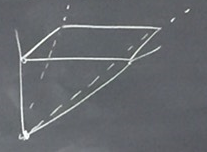
\includegraphics[width=0.5\textwidth]{pic/lec02pic01}
\end{figure}
\end{Eg}
\begin{Remark}
\begin{itemize}
\item $\sigma$ is a face of $\sigma$
\item the smallest face is
\begin{equation*}
\sigma\cap(-\sigma)(=\text{lineality space})
\end{equation*}
\item a face $\tau\leq\sigma$($\leq$ means a face of) is also a polyhedral cone. if $\sigma=\text{vcone}(A_1,\dots, A_n)$ and $u\in\sigma^{\vee}$, then $\tau=\text{vcone}(\{A_i:u\cdot A_i=0\})$.[\#o6 in hand out\#1:columns are gens of $\sigma$, rows are gens of $\sigma^{\vee}$, can figure out all faces($u_i^Tv_j=0$ in entry $(i,j)$)]
\end{itemize}
\end{Remark}

%---- Lecture 03 on Jan. 29th ---------
\newpage
\section{Lecture 03}

\begin{Def}
Let $\sigma \subseteq V$ be a polyhedral cone.
The following are equivalent:
\begin{enumerate}
\item $\sigma \cap (-\sigma) = \{0\}$
\item $\sigma$ contains no non-zero subspace
\item there exists $u \in \sigma^\vee$ such that $\sigma \cap u^\perp = \{0\}$
\item $\dim V = \dim \sigma^\vee$.
\end{enumerate}
If $\sigma$ satisfies the above than it is \emph{strongly convex} or \emph{pointed}.
\end{Def}

\begin{Def}
A \emph{face} of $\sigma$ is a subset $\tau \subseteq \sigma$ of the form $\tau = \sigma \cap u^\perp$ where $u \in \sigma^\vee$.
\end{Def}

Recall that if $\sigma$ is a polyhedral cone than $\mathrm{rel int}(\sigma)$ is the interior of $\sigma \subseteq(\mathrm{span}(\sigma))$ (except $\mathrm{rel int}(0) = 0$).
If $\sigma = \mathrm{vcone}(v_1, \dots, v_r)$ then $\mathrm{rel int}(\sigma) = \{\alpha_1v_1 + \dots + \alpha_rv_r : \alpha_i > 0\}$.

For the following facts let $\sigma = \mathrm{vcone}(v_1, \dots, v_r)$ and $\sigma^\vee = \mathrm{vcone}(u_1, \dots, u_s)$ be irredundant.

\begin{Fact}
Let $\tau_i = \sigma \cap u_i^\perp \subseteq \sigma$.
Then $\tau$ is a facet of $\sigma$.
\end{Fact}

\begin{Fact}
If $\mu = \mathrm{vcone}(u_{i1}, \dots, u_{il})$ is a face of $\sigma^\vee$ and $u \in \mathrm{rel int}(\mu)$ then
\[
\sigma \cap u^\perp = \bigcap_{j=1}^l(\sigma \cap u_{ij}^\perp) = \bigcap_{j=1}^l \tau_j.
\]
\end{Fact}

\begin{proof}
Since $u \in \mathrm{rel int}\mu)$ we have $u = \alpha_iu_{i1} + \dots + \alpha_lu_{il}$ where each $\alpha_j > 0$.
Let $v \in \sigma$.
Then $v \in \sigma \cap u^\perp$ if and only if $\langle u, v \rangle = 0$, which happens if and only if $\alpha_i\langle u_{i1}, v \rangle + \dots + \alpha_l\langle u_{il}, v \rangle = 0$.
But since $v \in \sigma$ we know $\langle u_j, v \rangle \le 0$ for all $u_j$, so this happens if and only if $\langle u_{ij}, v \rangle = 0$ for all $u_{ij}$.
This is equivalent to $v \in \bigcap_{j=1}^l \tau_{ij}$.
\end{proof}

\begin{Fact}
There is an order reversing bijection $\{\text{faces of $\sigma$}\} \to \{\text{faces of $\sigma^\vee$}\}$ given by $\tau \mapsto \sigma^\vee \cap \tau^\perp$ and (in reverse) $\tau^\star \mapsto \sigma \cap (\tau^\star)^\perp$.
For two elements in this bijection we have $\dim \tau + \dim \tau^\star = \dim V$.
\end{Fact}

\begin{Eg}
See the example from handout 1, where $\dim \sigma = 4$.
\end{Eg}

\begin{Def}
If $\sigma \subseteq V = \mathbb{R}^n$ and $\sigma$ is generated by vectors in $\mathbb{Q}^n$ (or equivalently $\mathbb{Z}^n$) we call $\sigma$ a \emph{rational} polyhedral cone.
\end{Def}

[NOTATION YOU DON'T WANT TO FORGET]

Let $M$ be a lattice (a finite abelian group with no torsion), so $M = \mathbb{Z}^n$ for some $n$.
We have
\[
M \subseteq M_{\mathbb{Q}} \subseteq M_{\mathbb{R}}
\]
where $M_k = M \otimes_{\mathbb{Z}} k$ so that $M = \mathbb{Z}^n$, $M_{\mathbb{Q}} = \mathbb{Q}^n$, and $M_{\mathbb{R}} = \mathbb{R}^n$.
Let $N$ be the dual lattice (so $N = \Hom(M, \mathbb{Z})$).
Choose dual coordinates
\[
e_1, \dots, e_n \quad \text{basis of $M$}
\]
\[
e_1^\star, \dots, e_n^\star \quad \text{dual basis of $N$}
\]
and define similarly $N \subseteq N_{\mathbb{Q}} \subseteq N_{\mathbb{R}}$.
Then $N_{\mathbb{Q}} = M_{\mathbb{Q}}^\star$ are dual vector spaces.
We will often use the notation ``$\sigma$ is a cone in $N$" to mean that $\sigma$ is a rational polyhedral cone in $N_{\mathbb{R}}$ (Fulton also adds to this definition that $\sigma^\vee$ is pointed).

\begin{Def}
If $M$ is a lattice then $S \subseteq M$ is a \emph{semigroup} if
\begin{enumerate}
\item $0 \in S$
\item if $m, m' \in S$ then $m + m' \in S$.
\end{enumerate}
\end{Def}

\begin{Eg}
$\mathbb{Z}^n$, $\mathbb{C}$ under multiplication, and $\mathbb{C}^\star$ are all semigroups.
\end{Eg}

\begin{Eg}
$S \subseteq \mathbb{Z}^2$ given by $S = \left\langle \begin{pmatrix}1\\1\end{pmatrix}, \begin{pmatrix}2\\1\end{pmatrix}, \begin{pmatrix}3\\1\end{pmatrix}, \dots \right\rangle$ is a semigroup that is not finitely generated.
\end{Eg}

\begin{Def}
If $\sigma$ is a cone in $N$ than $S_{\sigma} = \sigma^\vee \cap M$.
\end{Def}

(question: why not $S_\sigma = \sigma \cap N$?)

\begin{Eg}
Let $\sigma = \mathrm{vcone}\left(\begin{pmatrix}-2\\1\end{pmatrix}, \begin{pmatrix}0\\-1\end{pmatrix}\right)$.
Then $S_\sigma = \sigma^\vee \cap M = \left\langle \begin{pmatrix}1\\2\end{pmatrix}, \begin{pmatrix}1\\1\end{pmatrix}, \begin{pmatrix}1\\0\end{pmatrix} \right\rangle$.
\end{Eg}

\begin{Proposition}[Gordon's Lemma]
If $\sigma$ is a cone in $N$ then $S_\sigma$ is a finitely generated semigroup.
\end{Proposition}

\begin{proof}
Let $\sigma = \mathrm{vcone}(v_1, \dots, v_s)$ and let $K = \{\alpha_1v_1 + \dots + \alpha_sv_s : 0 \le \alpha_i < 1\}$.
Note that $K$ is bounded so $K \cap M$ is finite.
Clearly, $\sigma^\vee \cap M$ is generated by $v_1, \dots, v_s$ and $K \cap M$.
\end{proof}

\begin{Def}
Let $\sigma$ be a pointed cone in $N$.
Then $m \in \sigma^\vee \cap M = S_\sigma$ is called \emph{irreducible} if $m = m' + m''$ for $m', m'' \in S_\sigma$ means $m' = 0$ or $m'' = 0$.
\end{Def}

\begin{Proposition}
Let $H = \{m \in S_\sigma : \text{$m$ is irreducible}\}$.
Then
\begin{enumerate}
\item $H$ is finite
\item $H$ generates $S_\sigma$
\item every generating set of $S_\sigma$ contains $H$.
\end{enumerate}
\end{Proposition}

The set $H$ from the above proposition is the Hilbert basis of $S_\sigma$.

%---- Lecture 04 on Feb 5 ---------
\newpage
\section{Lecture 04}

Let $\sigma$ be a cone in $N$ (i.e., $\sigma$ is a rational, polyhedral, convex cone in $N_\mathbb{R}$).
Often $\sigma$ is pointed.
Recall that $S_\sigma = \sigma^\vee \cap M \subseteq M$ ($= \mathbb{Z}^n$) is a finitely generated semigroup by its Hilbert basis.

\begin{Def}
Let $A_\sigma = \CC[S_\sigma] = \CC[\sigma^\vee \cap M]$.
This is the $\CC$-algebra such that
\begin{enumerate}
\item $\{t^m : m \in S_\sigma\}$ is a $\CC$-basis for $A_\sigma$
\item $t^{m_1} \cdot t^{m_2} = t^{m_1 + m_2}$
\end{enumerate}
\end{Def}

\begin{Def}
$X_\sigma = \Spec A_\sigma$ is the \emph{affine toric variety} associated to $\sigma$.
\end{Def}

We want to understand:
\begin{itemize}
\item examples
\item ideal
\item points
\item tori and torus action
\item tangent space and singularities
\item toric morphisms.
\end{itemize}

Note that if $\sigma^\vee \cap M = \langle m_1, \dots, m_r \rangle$ then $A_\sigma$ is generated by $\{t^{m_1}, \dots, t^{m_r}\}$.
In particular, $A_\sigma$ is Noetherian.
We have an exact sequence
\[
0 \to \ker \phi \to \CC[x_1, \dots, x_r] \overset{\phi}{\to} A_\sigma \to 0
\]
where $\phi: x_i \mapsto t^{m_i}$.
Then defining $I_\sigma = \ker \phi$ gives that $A_\sigma = \CC[x_1, \dots, x_r]/I_\sigma$.
Thus $X_\sigma = V(I_\sigma) \subseteq \CC^r$ is an affine variety.

\begin{Eg}
Let $\sigma = \mathrm{vcone}\left(\begin{pmatrix}-1\\0\end{pmatrix}, \begin{pmatrix}0\\-1\end{pmatrix}\right)$.

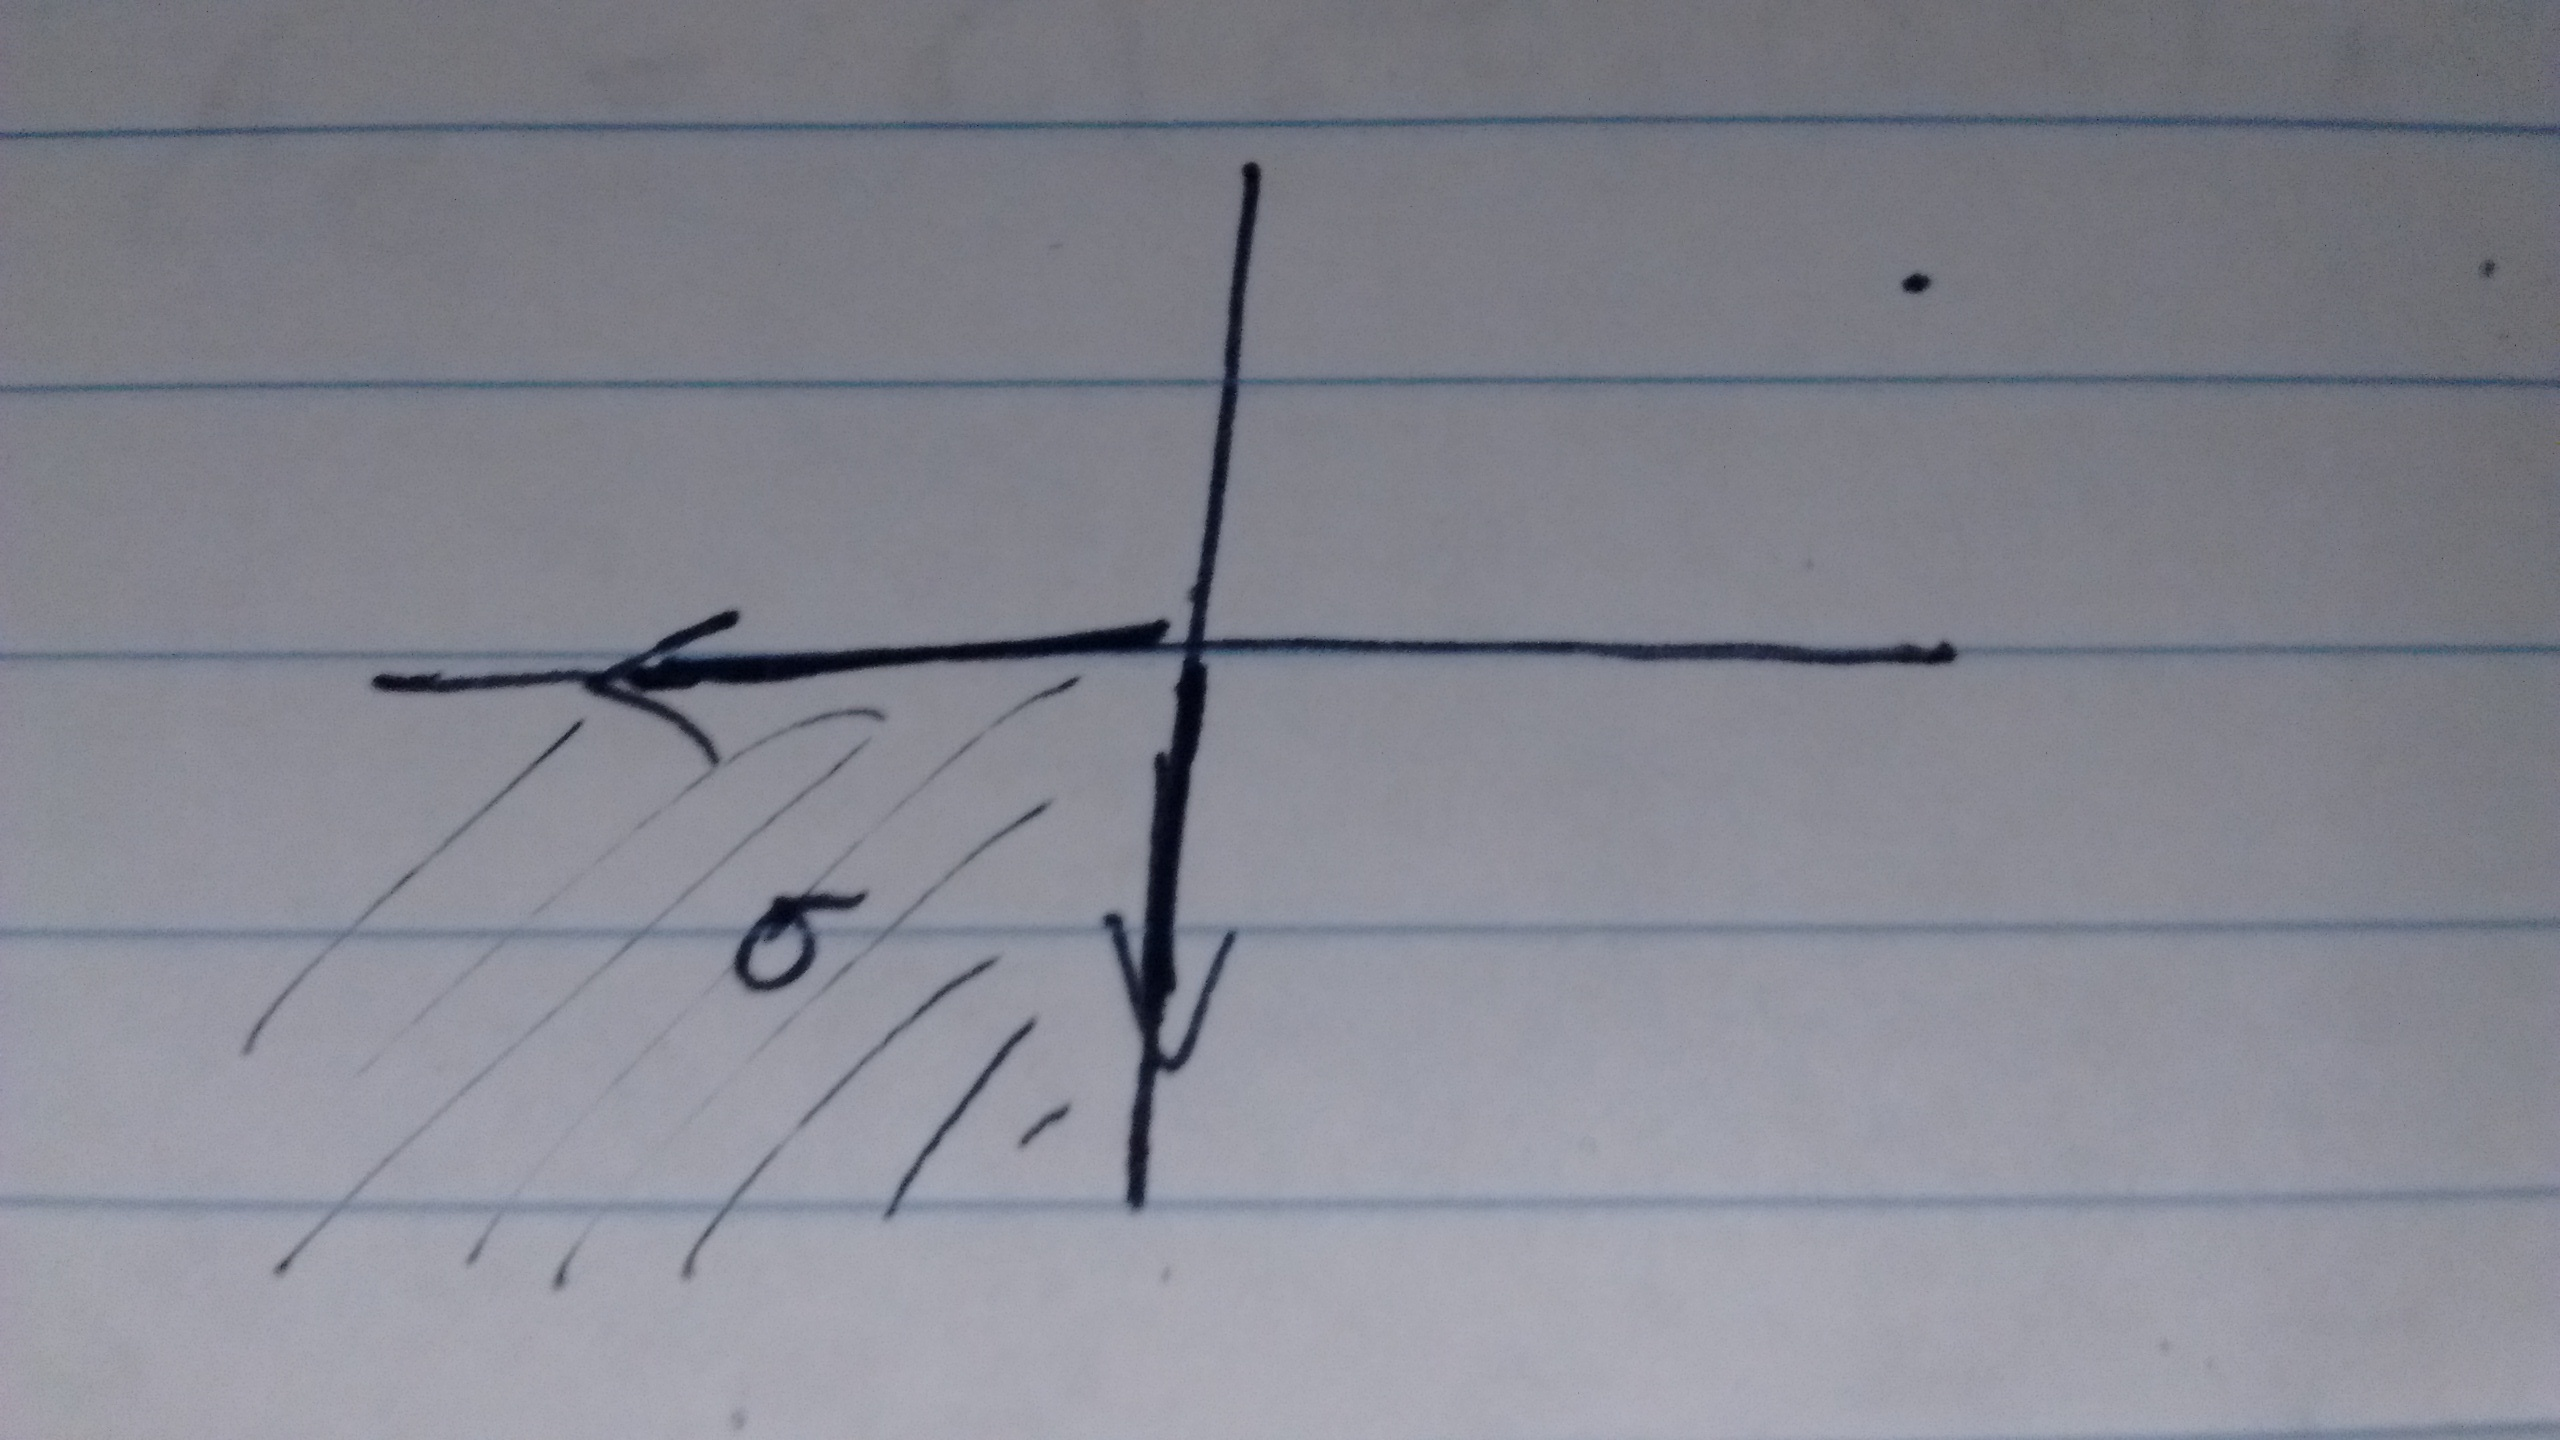
\includegraphics[width=0.3\textwidth]{pic/lec04-pic1}
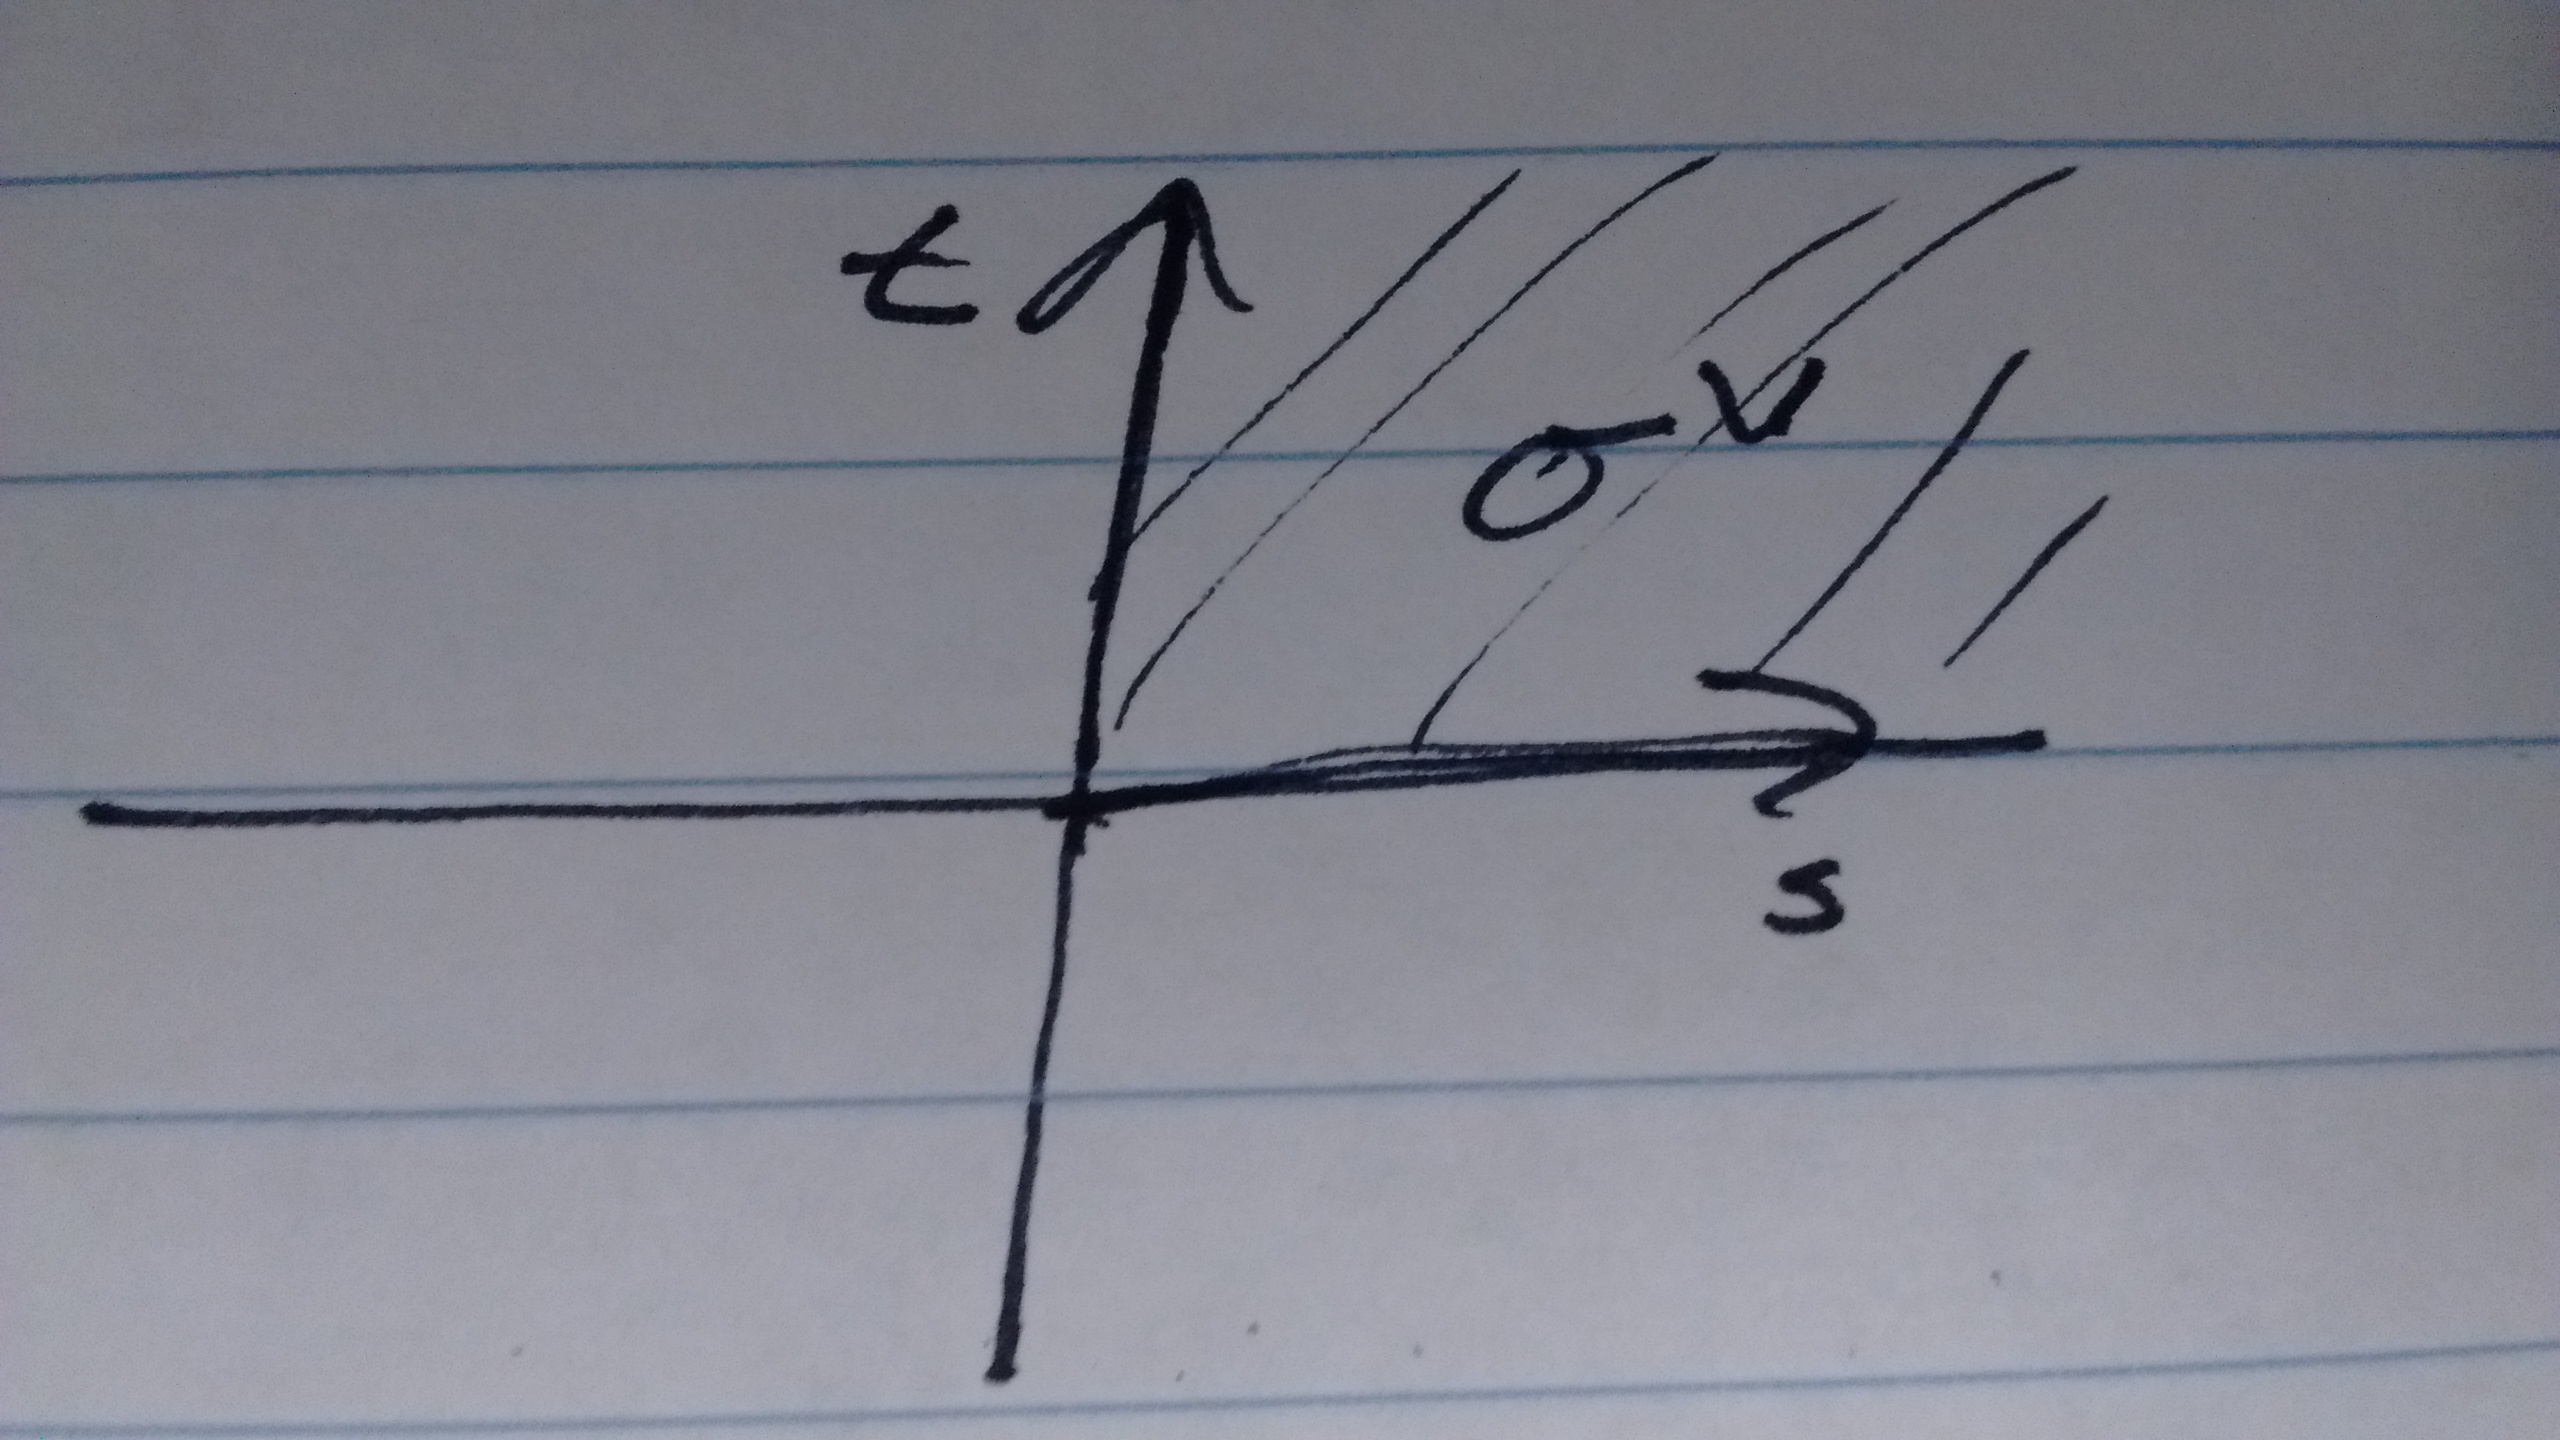
\includegraphics[width=0.3\textwidth]{pic/lec04-pic2}

Then $A_\sigma = \CC[s, t]$ and $X_\sigma = \CC^2$.
\end{Eg}

\begin{Eg}
If $\sigma = \mathrm{vcone}(-I_n) \subseteq \RR^n$ then $X_\sigma = \CC^n$.
If $\sigma = \mathrm{vcone}(I_n)$ then $X_\sigma = \CC^n$ but with different coordinates.
\end{Eg}

\begin{Eg}
Let $\sigma = \{0\}$ in $N = \ZZ^2$.
Then $\sigma^\vee = M_\RR$, $S_\sigma$ is all lattice points, and $A_\sigma = \CC[s,t,s^{-1},t^{-1}] = \CC[s, t]_{st}$.
This gives $X_\sigma = (\CC^\star)^2$, which is the algebraic torus $T$.
\end{Eg}

\begin{Eg}
Let $\sigma = \{0\}$ in $N = \ZZ^n$.
Then $\sigma^\vee = M_\RR$, $S_\sigma$ is all lattice points, and $A_\sigma = \CC[t_1^{\pm 1}, \dots, t_n^{\pm 1}]$.
This gives $X_\sigma = (\CC^\star)^n$, which is often denoted $T_n$.
\end{Eg}

\begin{Eg}
Let $\sigma = \mathrm{vcone}\left(\begin{pmatrix}-1\\2\end{pmatrix}, \begin{pmatrix}0\\-1\end{pmatrix}\right)$.
Then $\sigma^\vee = \mathrm{vcone}\left(\begin{pmatrix}2\\1\end{pmatrix}, \begin{pmatrix}1\\0\end{pmatrix}\right)$.

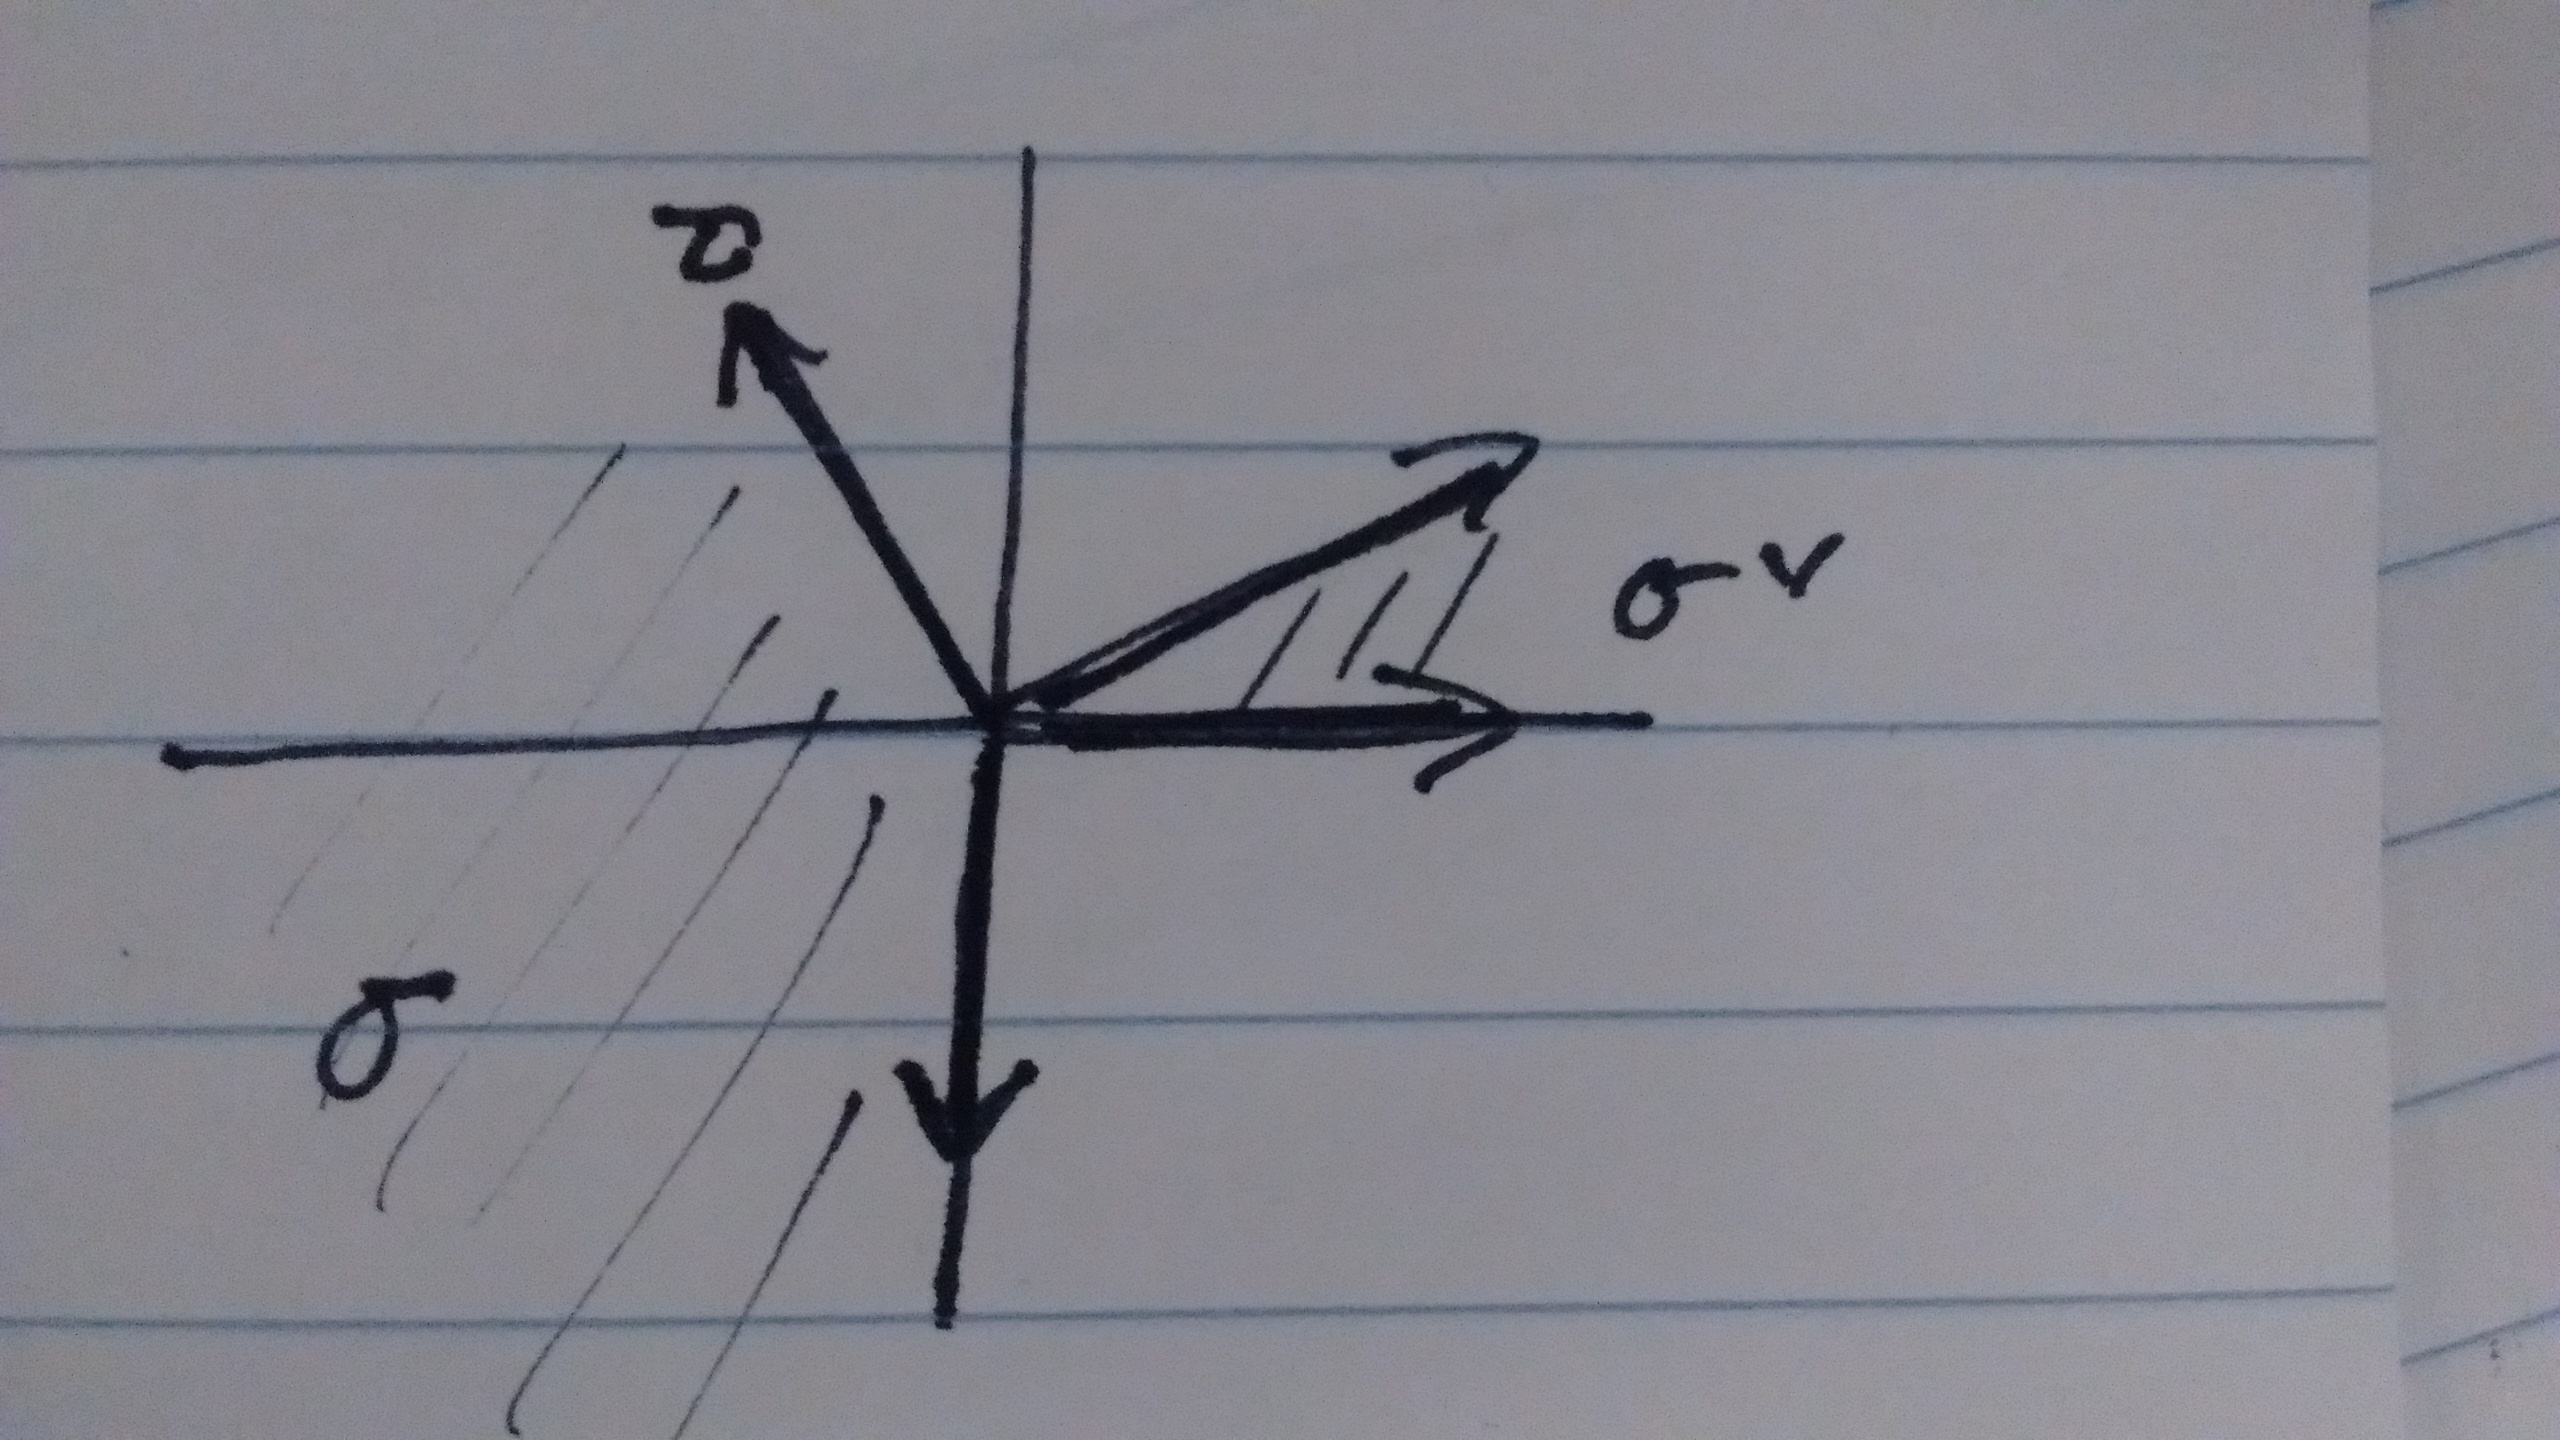
\includegraphics[width=0.3\textwidth]{pic/lec04-pic3}

We have $A_\sigma = \CC[s, s^2t] = \CC[u, v]$ and $X_\sigma = \CC^2$.

Now let $\tau = \mathrm{vcone}\left(\begin{pmatrix}-1\\2\end{pmatrix}\right)$ so $\tau^\vee = \mathrm{vcone}\left(\begin{pmatrix}2\\1\end{pmatrix}, \begin{pmatrix}-2\\1\end{pmatrix}, \begin{pmatrix}1\\0\end{pmatrix}\right)$.
Then $A_\tau = \CC[s^2t, (s^2t)^{-1}, s] = (A_\sigma)_{s^2t}$ and $X_\tau = \CC \times \CC^\star \hookrightarrow X_\sigma$ as an open set.
\end{Eg}

Exercise: If $\sigma$ is not pointed, what is $A_\sigma$ and $X_\sigma$?

As before, let $\sigma^\vee \cap M = \langle m_1, \dots, m_r \rangle$ and consider the exact sequence
\[
0 \to I_\sigma \to \CC[x_1, \dots, x_r] \overset{\phi}{\to} A_\sigma \to 0.
\]
Note that $A_\sigma = \CC[\sigma^\vee \cap M] \subseteq \CC[M] = \CC[t_1^{\pm 1}, \dots, t_n^{\pm 1}]$ and $\CC[t_1^{\pm 1}, \dots, t_n^{\pm 1}]$ is a domain.
Thus $A_\sigma$ is a domain, $I_\sigma$ is prime, and $X_\sigma$ is irreducible.

\end{document}
